\documentclass[tikz]{standalone}
\usetikzlibrary{calc, positioning, arrows.meta}

\def\s{s}  % server
\def\b{bot} % literal string
\tikzset{seq/.style = {draw, circle, outer sep = 5pt, inner sep = 2pt, scale = #1, left}}

% send: the sender sends operation to the receiver
\newcommand{\send}[5]{% #1: sender; #2: receiver; #3: sender pos; #4: receiver pos; #5: seq. number;
  \draw[->]  ($(#1)!#3!(#1\b)$) node[seq = 0.40] {#5} to ($(#2)!#4!(#2\b)$) node[seq = 0.60] {$#5$};
}

% csend: client sends operation to the server
\newcommand{\csend}[6]{% #1: client; #2: client pos; #3: server pos; #4: seq. number; #5: client state; #6: server state
  \draw[->]  ($(#1)!#2!(#1\b)$) node[seq = 0.60, fill = red!40, label = {[label distance = -6pt]-90:\fbox{$#5$}}] (#4) {#4}
    to ($(\s)!#3!(\s\b)$) node[seq = 0.50, label = {[label distance = -5pt, xshift = -1pt]-90:\fbox{$#6$}}] (server#4) {$#4$};
  % \send{#1}{\s}{#2}{#3}{#4}
}

% ssend: the server sends operation to client 
\newcommand{\ssend}[5]{% #1: client; #2: server pos; #3: client pos; #4: seq. number; #5: client state
  \draw[->, dashed]  ($(\s)!#2!(\s\b)$) to ($(#1)!#3!(#1\b)$) node[solid, seq = 0.50, 
	label = {[label distance = -5pt, xshift = -1pt]-90:\fbox{$#5$}}] (cl#4) {$#4$};
  % \send{\s}{#1}{#2}{#3}{#4}
}

\newcommand{\ins}[2]{$\textcolor{blue}{\textsc{Ins}(#1,#2)}$}
\newcommand{\del}[2]{$\textcolor{blue}{\textsc{Del}(#2)}$}  % del(a,p): ignoring the element 'a'

\begin{document}
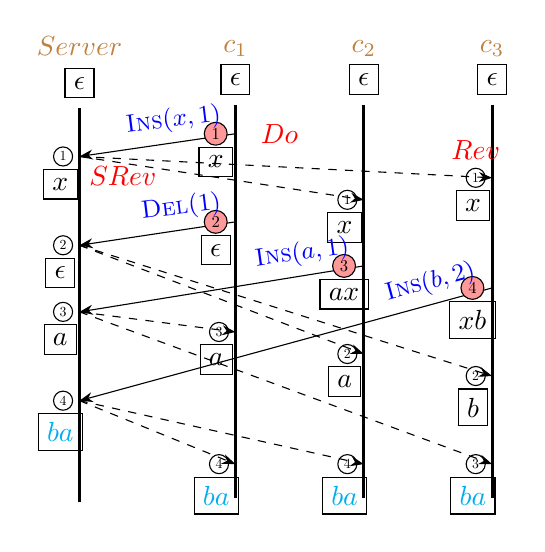
\begin{tikzpicture}[
    timeline/.style = {very thick}, >=Stealth, 
    op/.style = {font = \small, above left = -0.20cm and -0.40cm of #1, sloped},
    replica/.style = {align = center}]
  \node[replica] (\s) {\textcolor{brown}{$Server$} \\ \fbox{$\epsilon$}};
  \node[replica, right = of s] (c1) {$\textcolor{brown}{c_1}$ \\ \fbox{$\epsilon$}};
  \node[replica, right = of c1] (c2) {$\textcolor{brown}{c_2}$ \\ \fbox{$\epsilon$}};
  \node[replica, right = of c2] (c3) {$\textcolor{brown}{c_3}$ \\ \fbox{$\epsilon$}};

  \foreach \r/\rbot in {s/sbot, c1/c1bot, c2/c2bot, c3/c3bot} {
	\node[below = 5.0cm of \r] (\rbot) {};
	\draw[timeline] (\r) to (\rbot);
  }

  % send messages (ordered by positions at server)
  \csend{c1}{0.15}{0.20}{1}{x}{x}
  \node (o1) [op = {1}, rotate = 7] {\ins{x}{1}};
  \node (do) [right = 0.20cm of 1, red] {$Do$};
  \node (srev) [anchor = north, right = 0pt of server1, yshift = -7pt, red] {$SRev$};
  \ssend{c2}{0.20}{0.30}{1}{x}
  \ssend{c3}{0.20}{0.25}{1}{x}
  \node (rev) [anchor = north, above = 0pt of cl1, yshift = -3pt, red] {$Rev$};

  \csend{c1}{0.35}{0.40}{2}{\epsilon}{\epsilon}
  \node (o2) [op = {2}, rotate = 7] {\del{x}{1}};
  \ssend{c2}{0.40}{0.65}{2}{a}
  \ssend{c3}{0.40}{0.70}{2}{b}

  \csend{c2}{0.45}{0.55}{3}{ax}{a}
  \node (o3) [op = {3}, rotate = 8] {\ins{a}{1}};
  \ssend{c1}{0.55}{0.60}{3}{a}
  \ssend{c3}{0.55}{0.90}{3}{\textcolor{cyan}{ba}}

  \csend{c3}{0.50}{0.75}{4}{xb}{\textcolor{cyan}{ba}}
  \node (o4) [op = {4}, rotate = 15] {\ins{b}{2}};
  \ssend{c1}{0.75}{0.90}{4}{\textcolor{cyan}{ba}}
  \ssend{c2}{0.75}{0.90}{4}{\textcolor{cyan}{ba}}
\end{tikzpicture}
\end{document}
